% Тип документа
\documentclass[a4paper,12pt]{extarticle}

% Шрифты, кодировки, символьные таблицы, переносы
\usepackage{cmap}
\usepackage[T2A]{fontenc}
\usepackage[utf8x]{inputenc}
\usepackage[russian]{babel}

% Это пакет -- хитрый пакет, он нужен но не нужен
\usepackage[mode=buildnew]{standalone}

\usepackage
	{
		% Дополнения Американского математического общества (AMS)
		amssymb,
		amsfonts,
		amsmath,
		amsthm,
		% misccorr,
		% 
		% Графики и рисунки
		wrapfig,
		graphicx,
		subcaption,
		float,
		tikz,
		% tikz-3dplot,
		caption,
		csvsimple,
		color,
		booktabs,
		pgfplots,
		pgfplotstable,
		geometry,
		% 
		% Таблицы, списки
		makecell,
		multirow,
		indentfirst,
		%
		% Интегралы и прочие обозначения
		ulem,
		esint,
		esdiff,
		% 
		% Колонтитулы
		fancyhdr,
	}  


% Обводка текста в TikZ
\usepackage[outline]{contour}

% Увеличенный межстрочный интервал, французские пробелы
\linespread{1.3} 
\frenchspacing 

 
\usetikzlibrary
	{
		decorations.pathreplacing,
		decorations.pathmorphing,
		patterns,
		calc,
		scopes,
		arrows,
		fadings,
		through,
		shapes.misc,
		arrows.meta,
		3d,
		quotes,
		angles,
		babel
	}


\tikzset{
	force/.style=	{
		>=latex,
		draw=blue,
		fill=blue,
				 	}, 
	%				 	
	axis/.style=	{
		densely dashed,
		blue,
		line width=1pt,
		font=\small,
					},
	%
	th/.style=	{
		line width=1pt},
	%
	acceleration/.style={
		>=open triangle 60,
		draw=magenta,
		fill=magenta,
					},
	%
	inforce/.style=	{
		force,
		double equal sign distance=2pt,
					},
	%
	interface/.style={
		pattern = north east lines, 
		draw    = none, 
		pattern color=gray!60,
					},
	cross/.style=	{
		cross out, 
		draw=black, 
		minimum size=2*(#1-\pgflinewidth), 
		inner sep=0pt, outer sep=0pt,
					},
	%
	cargo/.style=	{
		rectangle, 
		fill=black!70, 
		inner sep=2.5mm,
					},
	%
	caption/.style= {
		midway,
		fill=white!20, 
		opacity=0.9
					},
	%
	}

\newenvironment{tikzpict}
    {
	    \begin{figure}[htbp]
		\centering
		\begin{tikzpicture}
    }
    { 
		\end{tikzpicture}
		% \caption{caption}
		% \label{fig:label}
		\end{figure}
    }


\newcommand{\vbLabel}[3]{\draw ($(#1,#2)+(0,5pt)$) -- ($(#1,#2)-(0,5pt)$) node[below]{#3}}
\newcommand{\vaLabel}[3]{\draw ($(#1,#2)+(0,5pt)$) node[above]{#3} -- ($(#1,#2)-(0,5pt)$) }

\newcommand{\hrLabel}[3]{\draw ($(#1,#2)+(5pt,0)$) -- ($(#1,#2)-(5pt,0)$) node[right, xshift=1em]{#3}}
\newcommand{\hlLabel}[3]{\draw ($(#1,#2)+(5pt,0)$) node[left, xshift=-1em]{#3} -- ($(#1,#2)-(5pt,0)$) }



\newcommand\zi{^{\,*}_i}
\newcommand\sumn{\sum_{i=1}^{N}}

\tikzset{
	coordsys/.style={scale=1.8,x={(1.1cm,-0cm)},y={(0.5cm,1cm)}, z={(0cm,0.8cm)}},
	coordsys/.style={scale=1.5,x={(0cm,0cm)},y={(1cm,0cm)}, z={(0cm,1cm)}}, 
	coordsys/.style={scale=1.5,x={(1cm,0cm)},y={(0cm,1cm)}, z={(0cm,0cm)}}, 
}

\usepgfplotslibrary{units}


% Draw line annotation
% Input:
%   #1 Line offset (optional)
%   #2 Line angle
%   #3 Line length
%   #5 Line label
% Example:
%   \lineann[1]{30}{2}{$L_1$}

\newcommand{\lineann}[4][0.5]{%
    \begin{scope}[rotate=#2, blue,inner sep=2pt, ]
        \draw[dashed, blue!40] (0,0) -- +(0,#1)
            node [coordinate, near end] (a) {};
        \draw[dashed, blue!40] (#3,0) -- +(0,#1)
            node [coordinate, near end] (b) {};
        \draw[|<->|] (a) -- node[fill=white, scale=0.8] {#4} (b);
    \end{scope}
}

\newcommand{\lineannn}[4][0.5]{%
    \begin{scope}[rotate=#2, blue,inner sep=2pt, ]
        \draw[dashed, blue!40] (0,0) -- +(0,#1)
            node [coordinate, near end] (a) {};
        \draw[dashed, blue!40] (#3,0) -- +(0,#1)
            node [coordinate, near end] (b) {};
        % \draw[color=white, color=blue] (a) -- node[fill=white, scale=0.8] {#4} (b);
        \draw[->|] (a)++(-0.3,0) -- (a);
        \draw[->|] (b)++(0.3,0) coordinate (xx) -- (b);
        \draw (xx) node[fill=white, scale=0.8, right] {#4};
    \end{scope}
}

% Круговая стрелка относительно центра (дуга из центра)
\tikzset{
  pics/carc/.style args={#1:#2:#3}{
    code={
      \draw[pic actions] (#1:#3) arc(#1:#2:#3);
    }
  },
  dash/.style={
  	dash pattern=on 5mm off 5mm
  }
}

% Среднее <#1>
\newcommand{\mean}[1]{\langle#1\rangle}

\pgfplotsset{
    % most recent feature set of pgfplots
    compat=newest,
}

% const прямым шрифтом
\newcommand\ct[1]{\text{\rmfamily\upshape #1}}
\newcommand*{\const}{\ct{const}}


\usepackage[europeanresistors,americaninductors]{circuitikz}

% Style to select only points from #1 to #2 (inclusive)
\pgfplotsset{select/.style 2 args={
    x filter/.code={
        \ifnum\coordindex<#1\def\pgfmathresult{}\fi
        \ifnum\coordindex>#2\def\pgfmathresult{}\fi
    }
}}


\usepackage{array}



%%%%%%%%%%%%%%%%%%%%%%%%%%%%%%%%%%%%%%%%%%%%%%%%%
\makeatletter
\newif\if@gather@prefix 
\preto\place@tag@gather{% 
  \if@gather@prefix\iftagsleft@ 
    \kern-\gdisplaywidth@ 
    \rlap{\gather@prefix}% 
    \kern\gdisplaywidth@ 
  \fi\fi 
} 
\appto\place@tag@gather{% 
  \if@gather@prefix\iftagsleft@\else 
    \kern-\displaywidth 
    \rlap{\gather@prefix}% 
    \kern\displaywidth 
  \fi\fi 
  \global\@gather@prefixfalse 
} 
\preto\place@tag{% 
  \if@gather@prefix\iftagsleft@ 
    \kern-\gdisplaywidth@ 
    \rlap{\gather@prefix}% 
    \kern\displaywidth@ 
  \fi\fi 
} 
\appto\place@tag{% 
  \if@gather@prefix\iftagsleft@\else 
    \kern-\displaywidth 
    \rlap{\gather@prefix}% 
    \kern\displaywidth 
  \fi\fi 
  \global\@gather@prefixfalse 
} 
\newcommand*{\beforetext}[1]{% 
  \ifmeasuring@\else
  \gdef\gather@prefix{#1}% 
  \global\@gather@prefixtrue 
  \fi
} 
\makeatother
%%%%%%%%%%%%%%%%%%%%%%%%%%%%%%%%%%%%%%%%%%%%%%%%%

\geometry		
	{
		left			=	2cm,
		right 			=	2cm,
		top 			=	3cm,
		bottom 			=	3cm,
		bindingoffset	=	0cm
	}

%%%%%%%%%%%%%%%%%%%%%%%%%%%%%%%%%%%%%%%%%%%%%%%%%%%%%%%%%%%%%%%%%%%%%%%%%%%%%%%



	%применим колонтитул к стилю страницы
\pagestyle{fancy} 
	%очистим "шапку" страницы
\fancyhead{} 
	%слева сверху на четных и справа на нечетных
\fancyhead[R]{\labauthors} 
	%справа сверху на четных и слева на нечетных
\fancyhead[L]{Отчёт по лабораторной работе №\labnumber} 
	%очистим "подвал" страницы
\fancyfoot{} 
	% номер страницы в нижнем колинтуле в центре
\fancyfoot[C]{\thepage} 

%%%%%%%%%%%%%%%%%%%%%%%%%%%%%%%%%%%%%%%%%%%%%%%%%%%%%%%%%%%%%%%%%%%%%%%%%%%%%%%

\renewcommand{\contentsname}{Оглавление}

\usepackage{tocloft}
% \renewcommand{\cftpartleader}{\cftdotfill{\cftdotsep}} % for parts
% \renewcommand{\cftsectiondotsep}{\cftdotsep}% Chapters should use dots in ToC
\renewcommand{\cftsecleader}{\cftdotfill{\cftdotsep}}
%\renewcommand{\cftsecleader}{\cftdotfill{\cftdotsep}} % for sections, if you really want! (It is default in report and book class (So you may not need it).
% ---------
% \newcommand{\cftchapaftersnum}{.}%
% \usepackage{titlesec}
% \titlelabel{\thetitle.\quad}
\usepackage{secdot}
\sectiondot{subsection}
\usepackage{setspace}
\usepackage{colortbl}
\usepackage{lscape}
\usepackage{booktabs,array}
\newcolumntype{C}{>{\centering\arraybackslash}m{5em}}

\def\labauthors{Понур К.А., Сарафанов Ф.Г., Сидоров Д.А.}
\def\labgroup{420}
\def\labnumber{211}
\def\labtheme{Продольные звуковые волны в проволоке}
\renewcommand{\vec}{\mathbf}
\renewcommand{\Re}{\operatorname{Re}}
\renewcommand{\Im}{\operatorname{Im}}
\renewcommand{\phi}{\phi}
\renewcommand{\kappa}{\varkappa}
\renewcommand{\hat}{\widehat}
\renewcommand{\epsilon}{\varepsilon}
\renewcommand{\phi}{\varphi}
\renewcommand{\d}{\partial}
\begin{document}

%%%%%%%%%%%%%%%%%%%%%%%%%%%%%%%%%%%%%%%%%%%%%%%%%%%%%%%%%%%%%%%%%%%%%%%%%%%%%%%
\begin{titlepage}

\begin{center}

{\small\textsc{Нижегородский государственный университет имени Н.\,И. Лобачевского}}
\vskip 1pt \hrule \vskip 3pt
{\small\textsc{Радиофизический факультет}}

\vfill

{\Large Отчет по лабораторной работе №\labnumber\vskip 12pt\bfseries \labtheme}
	
\end{center}

\vfill
	
\begin{flushright}
	{Выполнили студенты \labgroup\ группы\\ \labauthors}%\vskip 12pt Принял:\\ Менсов С.\,Н.}
\end{flushright}
	
\vfill
	
\begin{center}
	Нижний Новгород, \the\year
\end{center}

\end{titlepage}


%%%%%%%%%%%%%%%%%%%%%%%%%%%%%%%%%%%%%%%%%%%%%%%%%%%%%%%%%%%%%%%%%%%%%%%%%%%%%%%
\begin{spacing}{1}
\tableofcontents
\end{spacing}
% \setstretch{1.2}
\newpage
\section{Введение}
В работе изучается распространение продольных упругих волн в никелевой про волоке (диаметр проволоки мал по сравнению с длиной волны). Чтобы получить в нике левой проволоке длину волны порядка 1 см, необходимо для возбуждения применят! генератор с частотой порядка 500 кГц. Колебания такой частоты называют ультразвуко¬выми в отличие от колебаний звуковых частот, воспринимаемых ухом человека (верхней границей слухового восприятия считаются колебания с частотами около 20 кГц). Цель данной работы состоит в измерении длины возбуждаемой волны и скорости ее распро-странения.
\section{Продольные упругие волны}
В пренебрежении поглощением распространение продольных упругих волн в проволоке описывается волновым уравнением
\begin{equation}
\label{eq:1}
	\frac{\d^2s}{\d t^2}=\frac{E}{\rho}\frac{\d^2s}{\d x^2},
\end{equation}
где s(x,t)- смещение в момент t сечения, равновесная координата которого равна х ( х и
s отсчитываются вдоль оси, параллельной проволоке). Е и $\rho$ - соответственно модуль Юнга и плотность материала проволоки. Уравнение (\ref{eq:1}) справедливо при малых дефор¬мациях, лежащих в пределах применимости закона Гука. Общее решение этого уравнения представляет собой суперпозицию двух бегущих навстречу недеформирующихся волн:
\begin{gather*}
	s=s_1(x+ut)+s_2(x-ut),
\end{gather*}
где $u=\sqrt{E/\rho}$ - скорость распространения волны, $s_1$ $s_2$ - произвольные функции. Вид
функций $s_1$ и $s_2$ зависит от способа возбуждения волн и от граничных условий. Важен случай, когда $s_1$ и $s_2$ - плоские синусоидальные волны с циклической частотой $\omega$ и волновым числом $k$:
\begin{gather*}
	s_1=A+1\cos(\omega t+kx-\alpha_1), \\
	s_2=A_2\cos(\omega t -kx- \alpha_2)
\end{gather*}
Связь между $\omega$ и $k$ (дисперсионное уравнение) получим, подставляя любую из функций $s_1$ $s_2$, в уравнение (\ref{eq:1})
В рассматриваемом случае связь частоты волны с волновым числом линейная (скорость распространения волны и не зависит от частоты $\omega$), без свободного члена. Такие среды называются средами без дисперсии.

В нашей установке волны могут генерироваться в двух режимах: непрерывном и импульсном. В первом режиме непрерывно возбуждаются синусоидальные волны. Во втором режиме возбуждение синусоидальных волн периодически прерывается (генерируются обрывки синусоид - радиоимпульсы).

Рассмотрим суперпозицию двух плоских синусоидальных волн одинаковой амплитуды ($A_1=A_2=A$), распространяющихся во встречных направлениях:
\begin{gather*}
	s=s_1+s_2
\end{gather*}
Путем тригонометрических преобразований сумма двух гармоник может быть представлена в виде
\begin{equation}
\label{eq:2}
	s=2A\cos\left(kx-\frac{\alpha_1+\alpha2}{2}\right)\cos\left(\omega t+\frac{\alpha_1-\alpha_2}{2}\right),
\end{equation}
который описывает синусоидальную стоячую волну. Величина $s$ во всех точках струны совершает гармоническое колебание с одинаковой частотой, но амплитуда колебаний
\begin{gather*}
	2A\left|\cos\left(kx-\frac{\alpha_1+\alpha_2}{2} \right) \right|
\end{gather*}
различна в разных точках. Точки, где амплитуда равна нулю, и, следовательно, $s=0$ в любой момент времени, называются узлами стоячей волны. Точки, где амплигуда колебаний максимальна, называются пучностями стоячей волны.
 Амплитуда стоячей волны в пучности вдвое больше амплитуды каждой из бегущих волн. Расстояние между соседними пучностями, как и расстояние между соседними узлами, равно $\lambda/2$. Пучности и узлы сдвинуты друг относительно друга на четверть длины
волны.
Заметим, что множитель $\cos(kx)$ при переходе через нулевое значение меняет
знак, что соответствует изменению фазы колебаний на $\pi$. В соответствии с этим фаза колебаний по разные стороны от узла отличается на $\pi$. Точки, заключенные между двумя соседними узлами, колеблются синфазно.
Рассмотренный выше случай образования стоячей волны из двух бегущих навстречу волн является идеализированным. На практике получить чисто бегущую или чисто стоячую волну не удается. Причины этого состоят в следующем. Во-первых, вязкость (внутреннее трение) и теплообмен приводят к тому, что волна затухает при распространении, то есть энергия упругой волны переходит в тепловую. Во-вторых, отражение на границах проволоки в местах ее закрепления не полное. В результате мы имеем суперпозицию волн (излученной и отраженных) с разными амплитудами, и наблюдается режим смешанных волн. Рассмотрим поэтому более общий случай суперпозиции двух бегущих плоских волн одинаковой частоты с различными амплитудами, которые представим в виде:
\begin{gather*}
	A_2, A_1=A+a
\end{gather*}
Легко видеть, что $s=s_1+s_2$ есть суперпозиция стоячей волны, описываемой уравнением (\ref{eq:2}),  и бегущей волны
\begin{equation}
	a\cos(kx-\omega t-\alpha_1) \notag
\end{equation}
Величина $(a/A)^2$ называется коэффициентом бегучести. Отношение
\begin{equation}
	\frac{A_1^2+A_2^2}{A_1^2-A_2^2} \notag
\end{equation}
называется коэффициентом стоячести волны (КСВ). Очевидно, что в стоячей волне КСВ равен бесконечности, а в чисто бегузей -- единице.


\section{Метод возбуждения и приема упругих волн}

Известно, что под действием магнитного поля происходит деформация некоторых веществ (в частности, никеля). Это явление, открытое в середине прошлого века Джоулем получило название магнитострикции. Относительная деформация $\epsilon=\Delta L/L$ в полях, намагничивающих до насыщения ($H\approx10^5 A/m$), обычно исеет порядок $10^{-5}--10^{-6}$. Величина и знак деформации не зависит от направления магнитного полян, то есть функция $\epsilon(H)$- четная. Механизм магнитострикционныого эффекта нас в данной работе интересовать не будет; этот эффект используется лишь как способ получения ульразвуковых волн в проволоке.

Для возбужения упругих волн необходимо периодически измерять величину магнитого поля (в нашей установке магнитное поле меняется по гармоническому закону). Для достижения оптимальных условий возбуждения необходимо постоянное подмагничивание. В этом случае колебания $\epsilon(t)$ будут иметь максимальную возможную амплитуду, а их частота будет совпадать с частотой $H(t)$. Такая зависимость $\epsilon(H)$ характерна для никеля.

\section{Описание установки}

Установка состоит из передатчика, натянутой никелевой проволоки, передающей и приемной катушек, которые могут перемещаться вдоль проволоки, приемника и осциллографа. Передатчик и приемник собраны в одном корпусе.

Передатчик включает в себя: генератор высокой частоты, генерирующий непрерывное синусоидальное напряжение с частотой около 500 кГц; импульсный генератор, выдающий прямоугольные видеоимпульсы с периодом Т значительно большим времени длительности импульса $\tau$; при этом скважность $T/t$ оказывается достаточно большой; модулятор, являющийся своего рода "ключом": он пропускает синусоидальное напряжение голько в те моменты времени, когда одновременно с этим напряжением к нему приложено напряжение, снимаемое с выхода импульсного генератора. Таким образом, на выходе модулятора формируются радиоимпульсы, т.е. импульсы длительностью $\tau$ с синусоидальным заполнением, частота которого определяется частотой генератора высокой частоты; усилитель, усиливающий подводимое напряжение до величины, необходимой для нормальной работы передающей катушки.
С помощью переключателя "НЕПР-ИМП" напряжение ГВЧ подается или непосредственно на выходной усилитель (в этом случае установка будет работать в непрерывном режиме), или на модулятор (что обеспечивает имплльсный режим работы). Выходное напряжение снимается с разъема "Выход" (для удобства работы этот разъем запараллелен); к разъему "Видеоимпульс" подводится сигнал от испульсного генератора.

Для создания постоянного подмагничивания в месте расположения приемной и передающей катушек установлены постоянные магниты. Катушки секционированы, т.е.намотаны несколькими секциями; длина каждой секции порядка 2 мм. В месте расположения отдельных секций передающей катушки при подачи на неё переменного напряжения возникают упругие колебния. В приемной катушке переменное магнитное поле, возникающее из-за обратного магнитострикционного эффекта, создает ЭДС инжукции. Напряжение, снимаемое с этой катушки, поступает далее на разъем "Вход" приемника. Приемник представляет собой усилитель с полосой пропускания, достаточной для неискаженного усиления принимаемых сигналов. С выхода приемника усиленный сигнал поступает на вход вертикального усилителся осциллографа.

\section{Практическая часть}
\subsection{Импульсный режим}
% Было определено, что 
По осциллограммам была измерена длительность импульса $\tau=2*10^{-6}$ с, установлено, что $\tau_{radio}=\tau_{video}$  и определена величина $\frac{T}{\tau}$-- скважность:

\begin{gather*}
	\frac{T}{\tau}=77
\end{gather*}

По осциллограмме было определено, какой импульс пришел после отражения от одной стороны, другой стороны, и двух отражений.

Для определения скорости распространения волны было проведено два опыта с различным размещением приемника.

\begin{table}[H]
	    \caption{Результаты эксперимента}
	    \label{tab:chem1}
	    \pgfkeys{/pgf/number format/.cd,
		fixed,  1000 sep={\,}}
% \newlength\Colsep
% \setlength\Colsep{10pt}
% \xdef\Table{data/i.tsv}
	     % \xdef\C{5e-8}
% \xdef\R{13000}  
\pgfplotstableset{
	% multicolumn names, % allows to have multicolumn names
	% header=has colnames,
	dec sep align,
	col sep=tab, % the seperator in our .csv file
	fixed zerofill, 
	% precision=4,			
	columns/No/.style={
		column name={№},
		precision=0		
	},	
	columns/h/.style={
		column name={$h$, мм},
		% sci,
		precision=0,		
	},		
	columns/Nre/.style={
		column name={$N$, красный},
		% sci,
		precision=0,		
	},	
	columns/Ngr/.style={
		column name={$N$, зеленый},
		% sci,
		precision=0,		
	},	
	columns/Nwh/.style={
		column name={$N$, белый},
		% sci,
		precision=0,		
	},				
	columns/d/.style={
		column name={$d$, мм},
		% sci,
		precision=3,		
	},
	columns/r1/.style={
		column name={$r_1$, м},
		% sci,
		precision=3,		
	},
	columns/r2/.style={
		column name={$r_2$, м},
		% sci,
		precision=3,		
	},
	columns/r3/.style={
		column name={$r_3$, м},
		% sci,
		precision=3,		
	},
	columns/delta/.style={
		column name={$\delta$, мм},
		% sci,
		precision=3,		
	},
	columns/deltad/.style={
		column name={$\delta \cdot d$, мм},
		% sci,
		precision=3,		
	},
	columns/lambda/.style={
		column name={$\lambda$, нм},
		% sci,
		precision=0,		
	},
	columns/slambda/.style={
		column name={$\mean{\lambda}$, нм},
		% sci,
		precision=0,		
	},
	empty cells with={\textbf{--}},
	every head row/.style={
	before row={\toprule},
	after row={
		\midrule}
		},
	every last row/.style={after row=\bottomrule},
	every row/.style={after row=\midrule}, 
	columns={r1,r2,r3},	
	% dec zerofill
	% fixed,fixed zerofill,
	% precision=3
	% every even column/.style={
	% 	% column type/.add={>{\columncolor[gray]{.8}}}{}
	% },
	% every even row/.style={
	% 	before row={\rowcolor[gray]{0.95}}
	% },	
	}
	\centering
	\pgfplotstabletypeset[]{data/r.dat}

\end{table}

Здесь $r_1$ -- расстояние от крайней левой точки закрепления струны до передатчика, $r_2$ -- расстояние от передатчика до приемника и $r_3$ -- расстояние от приемника до крайней правой точки закрепления струны.

На приемнике детектируются и проходящие и отраженные волны, что приводит к тому, что наблюдается четыре пика на осциллограмме, соответствующих волне прошедшей непосредственно от передатчика к приемнику и других отраженных. Расстояния, пройденными этим волнами, нетрудно вывести:
\begin{gather}
\begin{aligned}
	s_1&=r_2\\
	s_2&=r_2+2r_3\\
	s_3&=2r_1+r_2\\
	s_4&=2r_1+r_2+2r_3\\
\end{aligned}
\end{gather}   

Здесь номер расстояния соответствует порядку следования пиков на экране осциллографа. 

Для снятых $r_1$ -- $r_3$ были рассчитаны $s_1$ -- $s_4$:
\begin{table}[H]
	    \caption{Результаты эксперимента}
	    \label{tab:chem1}
	    \pgfkeys{/pgf/number format/.cd,
		fixed,  1000 sep={\,}}
% \newlength\Colsep
% \setlength\Colsep{10pt}
% \xdef\Table{data/i.tsv}
	     % \xdef\C{5e-8}
% \xdef\R{13000}  
\pgfplotstableset{
	% multicolumn names, % allows to have multicolumn names
	% header=has colnames,
	dec sep align,
	col sep=tab, % the seperator in our .csv file
	fixed zerofill, 
	% precision=4,			
	columns/No/.style={
		column name={№},
		precision=0		
	},	
	columns/h/.style={
		column name={$h$, мм},
		% sci,
		precision=0,		
	},		
	columns/Nre/.style={
		column name={$N$, красный},
		% sci,
		precision=0,		
	},	
	columns/Ngr/.style={
		column name={$N$, зеленый},
		% sci,
		precision=0,		
	},	
	columns/Nwh/.style={
		column name={$N$, белый},
		% sci,
		precision=0,		
	},				
	columns/d/.style={
		column name={$d$, мм},
		% sci,
		precision=3,		
	},
	columns/S1/.style={
		column name={$s_1$, м},
		% sci,
		precision=3,		
	},
	columns/S2/.style={
		column name={$s_2$, м},
		% sci,
		precision=3,		
	},
	columns/S3/.style={
		column name={$s_3$, м},
		% sci,
		precision=3,		
	},
	columns/S4/.style={
		column name={$s_3$, м},
		% sci,
		precision=3,		
	},
	columns/delta/.style={
		column name={$\delta$, мм},
		% sci,
		precision=3,		
	},
	columns/deltad/.style={
		column name={$\delta \cdot d$, мм},
		% sci,
		precision=3,		
	},
	columns/lambda/.style={
		column name={$\lambda$, нм},
		% sci,
		precision=0,		
	},
	columns/slambda/.style={
		column name={$\mean{\lambda}$, нм},
		% sci,
		precision=0,		
	},
	empty cells with={\textbf{--}},
	every head row/.style={
	before row={\toprule},
	after row={
		\midrule}
		},
	every last row/.style={after row=\bottomrule},
	every row/.style={after row=\midrule}, 
	columns={S1,S2,S3,S4},
	% dec zerofill
	% fixed,fixed zerofill,
	% precision=3
	% every even column/.style={
	% 	% column type/.add={>{\columncolor[gray]{.8}}}{}
	% },
	% every even row/.style={
	% 	before row={\rowcolor[gray]{0.95}}
	% },	
	}
	\centering
	\pgfplotstabletypeset[]{data/s.dat}

\end{table}


Для каждого опыта посчитали скорость путем деления полного пути, пройденного волной, на полное время:

\begin{table}[H]
	    \caption{Первый опыт}
	    \label{tab:chem1}
	    \pgfkeys{/pgf/number format/.cd,
		fixed,  1000 sep={\,}}
% \newlength\Colsep
% \setlength\Colsep{10pt}
% \xdef\Table{data/i.tsv}
	     % \xdef\C{5e-8}
% \xdef\R{13000}  
% \pgfplotstableset{
% 	% multicolumn names, % allows to have multicolumn names
% 	% header=has colnames,
% 	dec sep align,
% 	col sep=tab, % the seperator in our .csv file
% 	fixed zerofill, 
% 	% precision=4,			
% 	columns/No/.style={
% 		column name={№},
% 		precision=0		
% 	},	
% 	columns/h/.style={
% 		column name={$h$, мм},
% 		% sci,
% 		precision=0,		
% 	},		
% 	columns/Nre/.style={
% 		column name={$N$, красный},
% 		% sci,
% 		precision=0,		
% 	},	
% 	columns/Ngr/.style={
% 		column name={$N$, зеленый},
% 		% sci,
% 		precision=0,		
% 	},	
% 	columns/Nwh/.style={
% 		column name={$N$, белый},
% 		% sci,
% 		precision=0,		
% 	},				
% 	columns/d/.style={
% 		column name={$d$, мм},
% 		% sci,
% 		precision=3,		
% 	},
% 	columns/S1/.style={
% 		column name={$s_1$, м},
% 		% sci,
% 		precision=3,		
% 	},
% 	columns/S2/.style={
% 		column name={$s_2$, м},
% 		% sci,
% 		precision=3,		
% 	},
% 	columns/S3/.style={
% 		column name={$s_3$, м},
% 		% sci,
% 		precision=3,		
% 	},
% 	columns/S4/.style={
% 		column name={$s_3$, м},
% 		% sci,
% 		precision=3,		
% 	},
% 	columns/delta/.style={
% 		column name={$\delta$, мм},
% 		% sci,
% 		precision=3,		
% 	},
% 	columns/deltad/.style={
% 		column name={$\delta \cdot d$, мм},
% 		% sci,
% 		precision=3,		
% 	},
% 	columns/lambda/.style={
% 		column name={$\lambda$, нм},
% 		% sci,
% 		precision=0,		
% 	},
% 	columns/slambda/.style={
% 		column name={$\mean{\lambda}$, нм},
% 		% sci,
% 		precision=0,		
% 	},
% 	empty cells with={\textbf{--}},
% 	every head row/.style={
% 	before row={\toprule},
% 	after row={
% 		\midrule}
% 		},
% 	every last row/.style={after row=\bottomrule},
% 	every row/.style={after row=\midrule}, 
% 	columns={S1,S2,S3,S4},
% 	% dec zerofill
% 	% fixed,fixed zerofill,
% 	% precision=3
% 	% every even column/.style={
% 	% 	% column type/.add={>{\columncolor[gray]{.8}}}{}
% 	% },
% 	% every even row/.style={
% 	% 	before row={\rowcolor[gray]{0.95}}
% 	% },	
% 	}
% 	\centering

	\pgfplotstabletypeset[
	columns/n/.style={
	string type, 
		column name={$i$},
		% sci,
		% precision=0,		
	},
	columns/S1/.style={
		column name={1},
		% sci,
		precision=3,		
	},
	columns/S2/.style={
		column name={2},
		% sci,
		precision=3,		
	},
	columns/S3/.style={
		column name={3},
		% sci,
		precision=3,		
	},
	columns/S4/.style={
		column name={4},
		% sci,
		precision=3,		
	},
	   every head row/.style={before row=\toprule, after row=\midrule},
	   every last row/.style={after row=\hline},
	% colnames from=Rank,
	% input colnames to=Rank
	]{data/o1.dat}\centering
	% \pgfplotstabletyp/eset[
	   % string type,
	   % every row 0 column Rank/.style={/pgfplots/table/@cell content/.add={\relax}{\cite{davis2007information}},},
	% ]{\loadedtable}
	% \pgfplotstabletypeset[]{data/s.dat}

\end{table}
\begin{table}[H]
	    \caption{Второй опыт}
	    \label{tab:chem1}
	    \pgfkeys{/pgf/number format/.cd,
		fixed,  1000 sep={\,}}
% \newlength\Colsep
% \setlength\Colsep{10pt}
% \xdef\Table{data/i.tsv}
	     % \xdef\C{5e-8}
% \xdef\R{13000}  
% \pgfplotstableset{
% 	% multicolumn names, % allows to have multicolumn names
% 	% header=has colnames,
% 	dec sep align,
% 	col sep=tab, % the seperator in our .csv file
% 	fixed zerofill, 
% 	% precision=4,			
% 	columns/No/.style={
% 		column name={№},
% 		precision=0		
% 	},	
% 	columns/h/.style={
% 		column name={$h$, мм},
% 		% sci,
% 		precision=0,		
% 	},		
% 	columns/Nre/.style={
% 		column name={$N$, красный},
% 		% sci,
% 		precision=0,		
% 	},	
% 	columns/Ngr/.style={
% 		column name={$N$, зеленый},
% 		% sci,
% 		precision=0,		
% 	},	
% 	columns/Nwh/.style={
% 		column name={$N$, белый},
% 		% sci,
% 		precision=0,		
% 	},				
% 	columns/d/.style={
% 		column name={$d$, мм},
% 		% sci,
% 		precision=3,		
% 	},
% 	columns/S1/.style={
% 		column name={$s_1$, м},
% 		% sci,
% 		precision=3,		
% 	},
% 	columns/S2/.style={
% 		column name={$s_2$, м},
% 		% sci,
% 		precision=3,		
% 	},
% 	columns/S3/.style={
% 		column name={$s_3$, м},
% 		% sci,
% 		precision=3,		
% 	},
% 	columns/S4/.style={
% 		column name={$s_3$, м},
% 		% sci,
% 		precision=3,		
% 	},
% 	columns/delta/.style={
% 		column name={$\delta$, мм},
% 		% sci,
% 		precision=3,		
% 	},
% 	columns/deltad/.style={
% 		column name={$\delta \cdot d$, мм},
% 		% sci,
% 		precision=3,		
% 	},
% 	columns/lambda/.style={
% 		column name={$\lambda$, нм},
% 		% sci,
% 		precision=0,		
% 	},
% 	columns/slambda/.style={
% 		column name={$\mean{\lambda}$, нм},
% 		% sci,
% 		precision=0,		
% 	},
% 	empty cells with={\textbf{--}},
% 	every head row/.style={
% 	before row={\toprule},
% 	after row={
% 		\midrule}
% 		},
% 	every last row/.style={after row=\bottomrule},
% 	every row/.style={after row=\midrule}, 
% 	columns={S1,S2,S3,S4},
% 	% dec zerofill
% 	% fixed,fixed zerofill,
% 	% precision=3
% 	% every even column/.style={
% 	% 	% column type/.add={>{\columncolor[gray]{.8}}}{}
% 	% },
% 	% every even row/.style={
% 	% 	before row={\rowcolor[gray]{0.95}}
% 	% },	
% 	}
% 	\centering

	\pgfplotstabletypeset[
	columns/n/.style={
	string type, 
		column name={$i$},
		% sci,
		% precision=0,		
	},
	columns/S1/.style={
		column name={1},
		% sci,
		precision=3,		
	},
	columns/S2/.style={
		column name={2},
		% sci,
		precision=3,		
	},
	columns/S3/.style={
		column name={3},
		% sci,
		precision=3,		
	},
	columns/S4/.style={
		column name={4},
		% sci,
		precision=3,		
	},
	   every head row/.style={before row=\toprule, after row=\midrule},
	   every last row/.style={after row=\hline},
	% colnames from=Rank,
	% input colnames to=Rank
	]{data/o2.dat}\centering
	% \pgfplotstabletyp/eset[
	   % string type,
	   % every row 0 column Rank/.style={/pgfplots/table/@cell content/.add={\relax}{\cite{davis2007information}},},
	% ]{\loadedtable}
	% \pgfplotstabletypeset[]{data/s.dat}

\end{table}

Значение скорости распространения волны, измеренное данным способом:
\begin{gather*}
	V=5.1\text{км/с}
\end{gather*}


При перемещении приемной катушки были зафиксированы сдвиги соответствующих импульсов относительно начального положения. Зная значения этих сдвигов по времени и расстоянию, можно так же оценить скорость распространения волны:

\begin{table}[H]
	    \caption{Разность двух опытов}
	    \label{tab:tab5}
	    \pgfkeys{/pgf/number format/.cd,
		fixed,  1000 sep={\,}}
% \newlength\Colsep
% \setlength\Colsep{10pt}
% \xdef\Table{data/i.tsv}
	     % \xdef\C{5e-8}
% \xdef\R{13000}  
% \pgfplotstableset{
% 	% multicolumn names, % allows to have multicolumn names
% 	% header=has colnames,
% 	dec sep align,
% 	col sep=tab, % the seperator in our .csv file
% 	fixed zerofill, 
% 	% precision=4,			
% 	columns/No/.style={
% 		column name={№},
% 		precision=0		
% 	},	
% 	columns/h/.style={
% 		column name={$h$, мм},
% 		% sci,
% 		precision=0,		
% 	},		
% 	columns/Nre/.style={
% 		column name={$N$, красный},
% 		% sci,
% 		precision=0,		
% 	},	
% 	columns/Ngr/.style={
% 		column name={$N$, зеленый},
% 		% sci,
% 		precision=0,		
% 	},	
% 	columns/Nwh/.style={
% 		column name={$N$, белый},
% 		% sci,
% 		precision=0,		
% 	},				
% 	columns/d/.style={
% 		column name={$d$, мм},
% 		% sci,
% 		precision=3,		
% 	},
% 	columns/S1/.style={
% 		column name={$s_1$, м},
% 		% sci,
% 		precision=3,		
% 	},
% 	columns/S2/.style={
% 		column name={$s_2$, м},
% 		% sci,
% 		precision=3,		
% 	},
% 	columns/S3/.style={
% 		column name={$s_3$, м},
% 		% sci,
% 		precision=3,		
% 	},
% 	columns/S4/.style={
% 		column name={$s_3$, м},
% 		% sci,
% 		precision=3,		
% 	},
% 	columns/delta/.style={
% 		column name={$\delta$, мм},
% 		% sci,
% 		precision=3,		
% 	},
% 	columns/deltad/.style={
% 		column name={$\delta \cdot d$, мм},
% 		% sci,
% 		precision=3,		
% 	},
% 	columns/lambda/.style={
% 		column name={$\lambda$, нм},
% 		% sci,
% 		precision=0,		
% 	},
% 	columns/slambda/.style={
% 		column name={$\mean{\lambda}$, нм},
% 		% sci,
% 		precision=0,		
% 	},
% 	empty cells with={\textbf{--}},
% 	every head row/.style={
% 	before row={\toprule},
% 	after row={
% 		\midrule}
% 		},
% 	every last row/.style={after row=\bottomrule},
% 	every row/.style={after row=\midrule}, 
% 	columns={S1,S2,S3,S4},
% 	% dec zerofill
% 	% fixed,fixed zerofill,
% 	% precision=3
% 	% every even column/.style={
% 	% 	% column type/.add={>{\columncolor[gray]{.8}}}{}
% 	% },
% 	% every even row/.style={
% 	% 	before row={\rowcolor[gray]{0.95}}
% 	% },	
% 	}
% 	\centering

	\pgfplotstabletypeset[
	columns/n/.style={
	string type, 
		column name={$i$},
		% sci,
		% precision=0,		
	},
	columns/S1/.style={
		column name={1},
		% sci,
		precision=3,		
	},
	columns/S2/.style={
		column name={2},
		% sci,
		precision=3,		
	},
	columns/S3/.style={
		column name={3},
		% sci,
		precision=3,		
	},
	columns/S4/.style={
		column name={4},
		% sci,
		precision=3,		
	},
	   every head row/.style={before row=\toprule, after row=\midrule},
	   every last row/.style={after row=\hline},
	% colnames from=Rank,
	% input colnames to=Rank
	]{data/do.dat}\centering
	% \pgfplotstabletyp/eset[
	   % string type,
	   % every row 0 column Rank/.style={/pgfplots/table/@cell content/.add={\relax}{\cite{davis2007information}},},
	% ]{\loadedtable}
	% \pgfplotstabletypeset[]{data/s.dat}

\end{table}

Значение скорости распространения волны, измеренное данным способом:
\begin{gather*}
	V=5\text{км/с}
\end{gather*}


\subsection{Непрерывный режим}

При включении непрерывного режима на экране осциллографа наблюдается полоса сигнала, меняющая свою ширину при перемещении принимающей катушки вдоль проволоки. Амплитуда колеблется от максимальных значений – <<пучности>>, до минимальных (ненулевых) – <<узлов>>. 

\subsubsection{Длина волны по амплитуде на осциллографе}

Для измерения длины волны нужно получить, на каком расстоянии $\Delta x$ находятся соседние пучности ($\Delta x = {\lambda\over2}$); для большей точности можно взять несколько (n=20) пучностей подряд. Передвигая катушку и отсчитывая пучности, дойдя до последней пучности, получаем $n/2$ длин волн, пройденных катушкой.

Найденная таким способом длина волны:
\begin{equation}
	\lambda=10.6 \text{ мм}
\end{equation}


\subsubsection{Зависимость КСВ от расстояния между приемником и передатчиком}

Коэффициент стоячести волны (КСВ) определим как отношение амплитуды в максимуме  $A_{max}$ к амплитуде в минимуме $A_{min}$:
\begin{equation}
 	\text{КСВ}=\frac{A_{max}^2+A_{min}^2}{A_{max}^2-A_{min}^2} \notag
 	% \frac{A_{max}}{A_{min}} \notag
\end{equation} 


\begin{figure}[H]
	\centering
	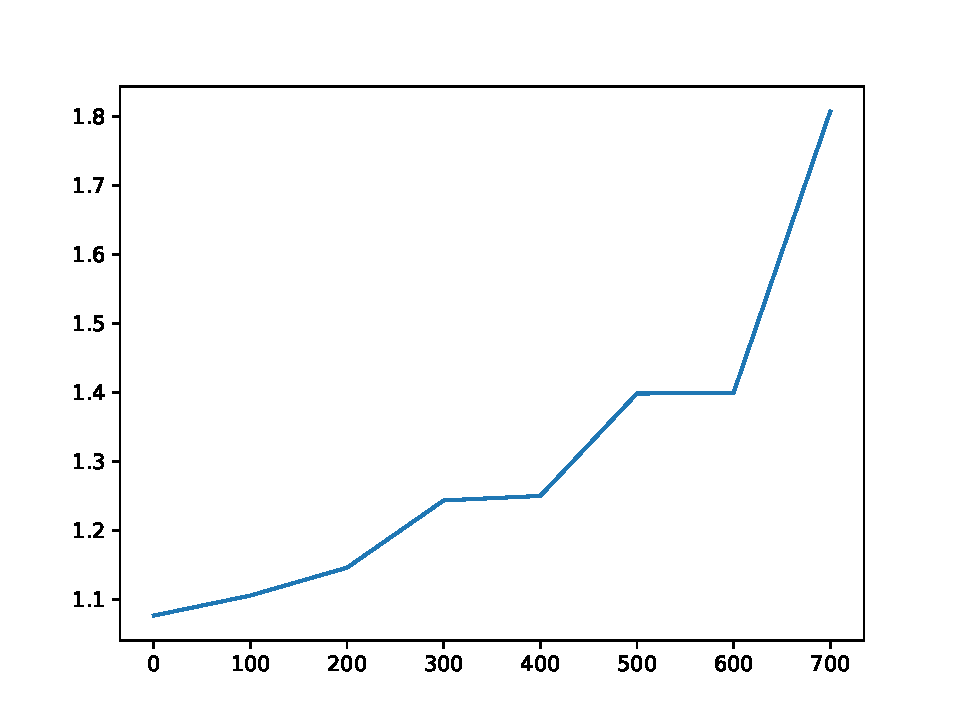
\includegraphics[width=0.8\textwidth]{fig1.pdf}
	\caption{Зависимость КСВ от от расстояния между приемником и передатчиком}
	\label{fig:1}
\end{figure}

\subsubsection{Длина волны по фигуре Лиссажу на осциллографе}

Второй способ измерений заключается в подаче сигнала с генератора и с приемника на осциллограф, где наблюдается фигура Лиссажу - эллипс. 

Вырождение в прямую соответствует узлам(в зависимости от наклона прямой), таким образом, зафиксировав одно из положений прямой и двигая приемник, можно дойти до следующего такого же изображения на осциллографе, это будет соответствовать передвижению приемника на длину волны.

Найденная таким способом длина волны:
\begin{equation}
	\lambda=10.65 \text{ мм}
\end{equation}
% Также была зафиксирована фаза принимаемого сигнала в зависимости от положения катушки. На второй вход осциллографа был подан сигнал непосредственно с генератора, в следствии чего на экране наблюдалась фигура Лиссажу (эллипс). Перемещая приемник, и фиксируя количество одинаковых положений также была посчитана длина волны:


% \subsection{Погрешности}
% $\Delta x=0.1$ см -- для измерений расстояния

% $\Delta A=0.08$ В -- для измерений амплитуд
\end{document} 